\chapter{Applikation}
Die Applikation soll die Verwendung vom TIMA ohne Webbrowser, für möglichst
viele Endnutzer möglich machen.  Besonders für Mobile Geräte soll die Nutzung
vereinfacht werden.\\ Als erste Variante wurden grundlegende Funktionen der
Webseite nachgebaut.  Dies diente auch der Entwicklung dieser, um etwaige
Fehler im Protokoll oder Verbesserungen dessen aufzuzeigen.

\section{Framework}
Als Framework wurde sich für Qt5 entschieden Aufgrund der weitreichenden
Unterstützung des Frameworks von Endgeräten.\\ Es wurde zudem Java in betracht
bezogen, da dies vorrangig auf Mobilen Geräten Verwendung findet. Allerdings
wurde sich aus Sympathiegründen des Entwicklers dagegen entschieden.

\section{Aufbau}
Die innere Logik wird durch einen Zustandsautomaten dargestellt um
Mehrfachanfragen zu vermeiden und eine einfache Fehlerkerrektur zu ermöglichen.
In Abbildung \ref{fig:uml_automata} wird der zusammenhang der einzelnen
Zustände angezeigt. Das wechseln der Zustände wir rein über die Qt eigenen
Signale geregelt.
\begin{figure}[!h]
	\centering
	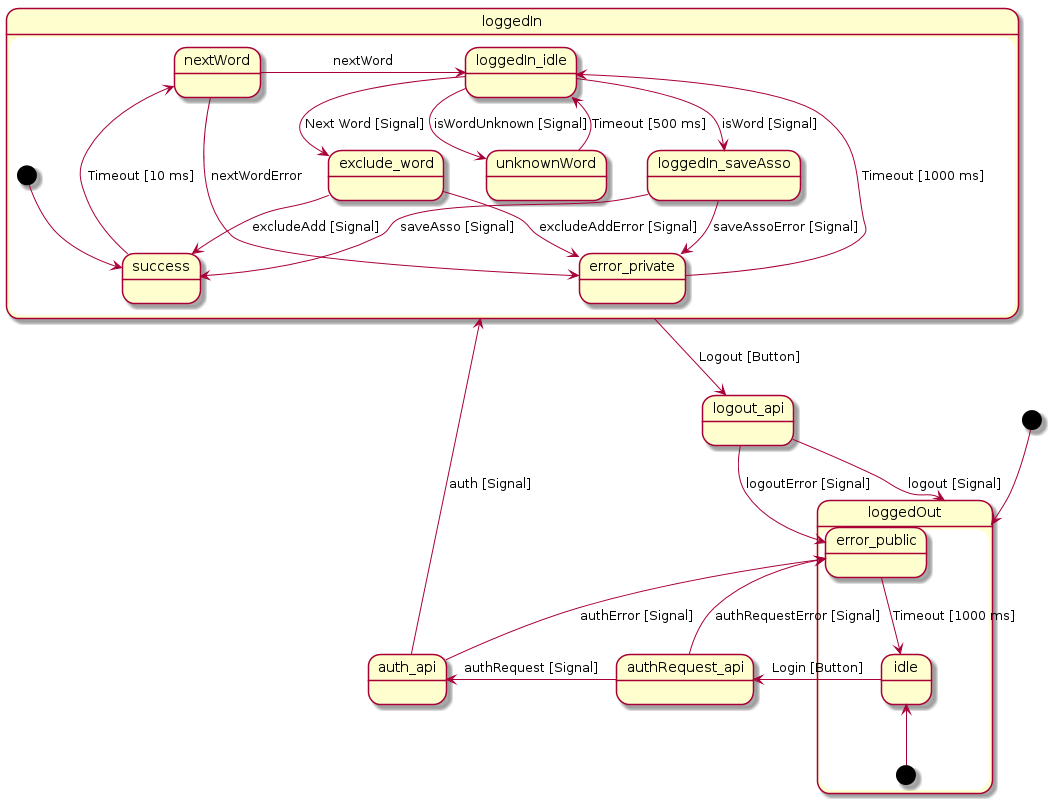
\includegraphics[width=\textwidth]{../UML/app_automata.png}
	\caption{UML State Diagramm des Applikations Zustandsautomaten}
	\label{fig:uml_automata}
\end{figure}

\section{Sicherheit}
Die Sicherheit hat bei der Entwicklung eine Große Rolle gespielt.  Auch wenn
das Projekt nicht unbedingt einer größeren Sicherheitsvorkehrung als SSL
bedürfte, wurde sich für die Absicherung von Teilen der API durch
unauthorisierte Dritte Abgesichert. Dies dient dazu, lediglich von TIMA
akzeptierte Programme schreibrechte für die Datenbank zu geben.  Das Auslesen
der Informationen bliebt jedoch davon unangetastet und ist nach wie vor für
jeden offen.

\subsection*{Sicherheitsplanung}
In der ersten Version wurde eine Verschlüsselung mit PGP geplant um eine
vollständige \glqq Ende zu Ende\grqq~Verbindung herzustellen und auch \glqq Man
in the Middle\grqq~Atacken auszuschließen. Doch aufgrund von erhöhtem
Programmieraufwand wurde hierauf verzichtet.\\

In der zweiten Version wurde eine Implementierung vom OAUTH2 Standart versucht.
Die Anforderungen bestanden hierbei an einem geheimen Schlüssel in der
Applikation, einem Auschluss einer Replay-Atacke und dem Verwenden von
User eigenen Passwörtern.\\
Im Standart sind 4 verschiedene \glqq Authorization Grants\grqq~
definiert\footnote{siehe \url{https://tools.ietf.org/html/rfc6749\#section-1.3}}
jedoch erfüllt keine davon jede Anforderung an das gewünschte Protokoll.\\

Der Dritte Versuch ist eine Eigenentwicklung um sowohl den Arbeitsaufwand
klein zu halten, als auch alle Anforderungen ausreichend zu erfüllen.
Eine kleine Übersicht ist in Abbildung \ref{fig:uml} zu sehen.\\
Die Übertragung erfolgt mit JSON Objekten um das Parsen zu erleichtern und
einen üblichen Standart zu verwenden. Der Rechenaufwand des Servers wurde
zudem versucht so gering wie möglich zu halten, um mögliche DDOS Angriffe
anzuschwächen.

\subsection{Authentisierung}
Eine Authentisierung ist wie folgt aufgebaut.
Der Client sendet eine Authentisierungsanfrage an den Server mit seinem
Benutzernamen und einer Applikations-Identifikationsnummer. Der Nutzername
dient dem Server zur Zuordnung zum Benutzerprofil und die Identifikationsnummer
regelt die Zugehörigkeit der verwendeten Applikation. Es werden nur registrierte
Applikationen akzeptiert.\\
Bei korrekten Informationen sendet der Server seine aktuelle Uhrzeit zurück
und speichert diese unter dem angegebenen Nutzerprofil ab. Dieser Zeitstempel
wird für die Signierung der weiteren Pakete verwendet und um nicht wiederkehrende
Signaturen zu erzwingen.\\
Im nächsten Schritt erstellt der Client das eigentliche Authentisierungs Paket mit
seinem Benutzernamen, seinem Passwort, der Identifikationsnummer, dem Zeitstempel
und einem Token als Signatur, welcher aus dem Hash des Zeitstempels und dem
konkatinierten Applikations-Geheimnis besteht. Als Hashmethode wurde hierbei
SHA-512 verwendet.\\
Nachdem der Server alle Angaben überprüft hat und die Signatur korrekt
verifizieren konnte, erhält er eine laufende Paketnummer, einen für ihn
geltende Benutzer-Identifikationsnummer und einen Usertoken.\\
Für jede weitere API Abfrage muss mindestens die Benutzer-Identifikationsnummer
und eine Signatur bestehend aus dem SHA-512 Hash des Usertoken konkatiniert mit
der Paketnummer verschickt werden. Nach jeder erfolgreichen API Anfrage welche
die Paketnummer und die Signatur verlangt, wird die Paketnummer um eins erhöht.
Aus Kompatibilitätsgründen läuft die Paketnummer bis maximal 2147483646 und
fängt danach wieder bei 0 an.


\section{Spiele}
Um mehr Nutzer zu erziehlen sind verschiedene Spiele geplant worden, die jedoch
aus Zeitgründen nicht in den geplanten Zeitrahmen passten.

Als Grundlage wird jedoch in den meißten Fällen schon eine gut gefüllte Datenbank
vorrausgesetzt.\\

Die einzelnen Spiele sind
\begin{itemize}
  \item Familienduell
  \item Assoziationskette (Einzelspieler)
  \item Assoziationskette (Mehrspieler)
\end{itemize}

\subsection*{Familienduell}
Da dieses Spiel die größte Beliebtheit verspricht, sei hier noch einmal kurz
die Funktionsweise erklärt.\\
Der Name soll hierbei nur die Ausrichtung des Spieles näher bringen.
Wie bei der
Fernsehserie\footnote{siehe \url{https://de.wikipedia.org/wiki/Familien-Duell}},
werden Dem Benutzer verschiedene verdeckte Antworten auf eine Frage gezeigt
und für jede richtig gegebene Antwort erhält der Spieler Punkte.
Die Fragen sind jedoch ausschließlich die meißt genannten Assoziationen zu einem
bestimmten Wort. Zusätzlich sollte eine Zeitbegrenzung eingehalten werden, da ja
alle Korrekten Antworten auf TIMA nachgeschaut werden können.























